\documentclass{article}
\usepackage[landscape]{geometry}
\usepackage{url}
\usepackage{multicol}
\usepackage{amsmath}
\usepackage{amsfonts}
\usepackage{bm}
\usepackage{tikz}
\usetikzlibrary{decorations.pathmorphing}
\usepackage{amsmath,amssymb}
\usepackage{tabularx,ragged2e,booktabs,caption}
\usepackage{colortbl}
\usepackage{xcolor}
\usepackage{mathtools}
\usepackage{amsmath,amssymb}
\usepackage{enumitem}
\usepackage[parfill]{parskip}

\title{Case Study}
\usepackage[brazilian]{babel}
\usepackage[utf8]{inputenc}

\advance\topmargin-.8in
\advance\textheight3in
\advance\textwidth3in
\advance\oddsidemargin-1.5in
\advance\evensidemargin-1.5in
\parindent0pt
\parskip2pt
\newcommand{\hr}{\centerline{\rule{3.5in}{1pt}}}

\begin{document}

\begin{center}{\huge{\textbf{Latent Factor Modeling of Lymphoma Survival Times}}}\\
\vspace{1mm}
{\large By Steve Kang, Sam Yin, Lucy Lu}
\end{center}
\begin{multicols*}{3}

\tikzstyle{mybox} = [draw=black, fill=white, very thick, rectangle, rounded corners, inner sep=10pt, inner ysep=10pt]
\tikzstyle{fancytitle} = [fill=black, text=white, font=\bfseries]

\begin{tikzpicture}
\node [mybox] (box){
    \begin{minipage}{0.3\textwidth}
    In this case study, we examine length of survival and gene expression levels for 240 subjects. In order to reduce number of covariates, we first conduct independent screening with Cox proportional model. Afterwards, we impute censored data with a Gibbs Sampler. As for modeling and prediction, we use both Unweighted and Weighted Latent Factor Models with 9 latent factors. The result indicates that Unweighted Latent Factor Model performs the best by root mean squared error (RMSE).
    \end{minipage}
};

\node[fancytitle, right=10pt] at (box.north west) {Abstract};
\end{tikzpicture}


\begin{tikzpicture}
\node [mybox] (box){
    \begin{minipage}{0.3\textwidth}
		The large number of predictors (7,399 gene expression levels) in this data set necessitates variable selection. Independent screening with Cox proportional hazard model is applied for each covariate: 
        \begin{equation*}
        \lambda_i(t) = \lambda_{0}(t)\exp(\beta_jx_{ij}), \ i = 1, ..., n,\ j = 1, ..., m
        \end{equation*}
		where $\lambda_i(t)$ is the hazard rate for subject $i$ at time $t$\, $\lambda_{0}(t)$ is the baseline hazard when no effect of explanatory variable (gene expression levels) is present, and $\beta_j$ is the coefficient for $x_{ij}$, the $j^{th}$ gene of subject $i$. 
    
		The threshold for variable selection is determined by False Discovery Rate (FDR) correction which controls for the overall Type I error rate in multiple comparisons. The procedure (also referred to as Benjamini–Hochberg procedure) is as follows: 
        \begin{enumerate}
        \item Sort the p-values $p_{1}, p_{2}, \ldots, p_{m}$ for all $m$ models in ascending order; \\
        \item For $\alpha = 0.05$, find the largest $k$ such that $p_{k} \leq \frac{k}{m} \alpha$; \\
        \item Reject the null hypotheses corresponding to $p_{1}, p_{2}, \ldots, p_{k}$, i.e., select the first $k$ corresponding predictors.
        \end{enumerate}
        
        The above procedure identifies 77 genes which will be used in imputation and modeling.
    \end{minipage}
};

\node[fancytitle, right=10pt] at (box.north west) {Independent Screening};
\end{tikzpicture}


\begin{tikzpicture}
\node [mybox] (box){
    \begin{minipage}{0.3\textwidth}
    The follow-up period in the original study was not able to cover the life span of many patients. As a result, the survival time of 102 out of 240 subjects are right-censored. The following Gibbs sampler is used for data imputation: 
    for $t = 1, 2, \ldots, T$
    \begin{enumerate}
    \item Sample $\tilde{Y}_{i}^{(t)} \sim TruncNorm(\bm{\beta}^{T}\mathbf{X}_{i}, \tau^{-1}; L = \tilde{Y}_{i}^{(0)})$ for all censored $Y_{i}$'s (where $\tilde{Y}_{i}^{(0)}$ is based on the observed survival time), \\
    \item Update $\bm{\beta} \sim MVN(\Sigma(\Sigma_{0}^{-1}\bm{\beta} + \tau\mathbf{X}^{T}\mathbf{Y}), \Sigma)$ where $\Sigma = (\Sigma_{0}^{-1} + \tau\mathbf{X}^{T}\mathbf{X})^{-1}$ and $\tau \sim Gamma(a + \frac{n}{2}, b + \frac{1}{2}(\mathbf{Y} - \mathbf{X}\bm{\beta})^{T}(\mathbf{Y} - \mathbf{X}\bm{\beta}))$. 
    \end{enumerate}
    
    The parameters are initialized as $\bm{\beta} \sim MVN(\bm{\beta}_{0}, \Sigma_{0})$ and $\tau \sim Gamma(a, b)$ where $\bm{\beta}_{0} = \mathbf{0}, \Sigma_{0} = \mathcal{I}, a = b = 1$. The median of the sampled $\mathbf{Y}_{i}^{(t)}$'s are imputed.
    \end{minipage}
};

\node[fancytitle, right=10pt] at (box.north west) {Data Imputation};
\end{tikzpicture}


\begin{tikzpicture}
\node [mybox] (box){
    \begin{minipage}{0.3\textwidth}
	Assume that several groups of correlated genes form pathways ``meta genes" and collectively affect the survival time of subjects. These pathways can be modeled as k latent factors (k $<<$ p, where p is the number of explanatory variables in the original data set), and the covariance matrix of $\mathbf{X}$ can be decomposed as $\Sigma = \Lambda\Lambda^{T} + \Psi$ where $\Lambda$ has dimension $p \times k$ and $\Psi$ is a $p \times p$ diagonal matrix. Given the latent factors, the gene expression levels and the survival time are conditionally independent. \\
    This latent factor model is formulated as follows: \\
    $$x_{ij} = \lambda_{j}\eta_{i} + \epsilon_{ij}, \epsilon_{ij} \sim N(0, \phi_{j}),$$
    $$y_{i} = \alpha + \eta_{i}^{T}\beta + \nu_{i}, \nu_{i} \sim N(0, \sigma^{2}),$$
    where $y_{i}$ is the log survival time of the $i^{\text{th}}$ subject, $\lambda_{j}$ is the $j^{\text{th}}$ row of the factor loading matrix $\Lambda$, $\eta_{i}$ is the level of latent factors for the $i^{\text{th}}$ subject. One modification to the likelihood function is upweighting $y_{i}$: $\mathcal{L}(\mathbf{X}, \mathbf{Y}|-) = \prod_{i = 1}^{n}\{[\prod_{j = 1}^{p}(P(X_{ij}|-))]P(\log(Y_{i})|-)^{w}\} (w \geq 1).$ \\
    The model was implemented with JAGS package in RStudio. The training set consists of the first 160 subjects, and the test set the other 80. The prediction of log survival time is based on the posterior means of parameters. $\hat{Y} \sim N(\hat{\alpha} + \mathbf{X}\hat{\Lambda}(\hat{\Lambda}^{T}\hat{\Lambda})^{-1}\hat{\beta}, \hat{\sigma}^{2})$.
    \end{minipage}
};

\node[fancytitle, right=10pt] at (box.north west) {Latent Factor Model};
\end{tikzpicture}

\begin{tikzpicture}
\node [mybox] (box){%
    \begin{minipage}{0.3\textwidth}
    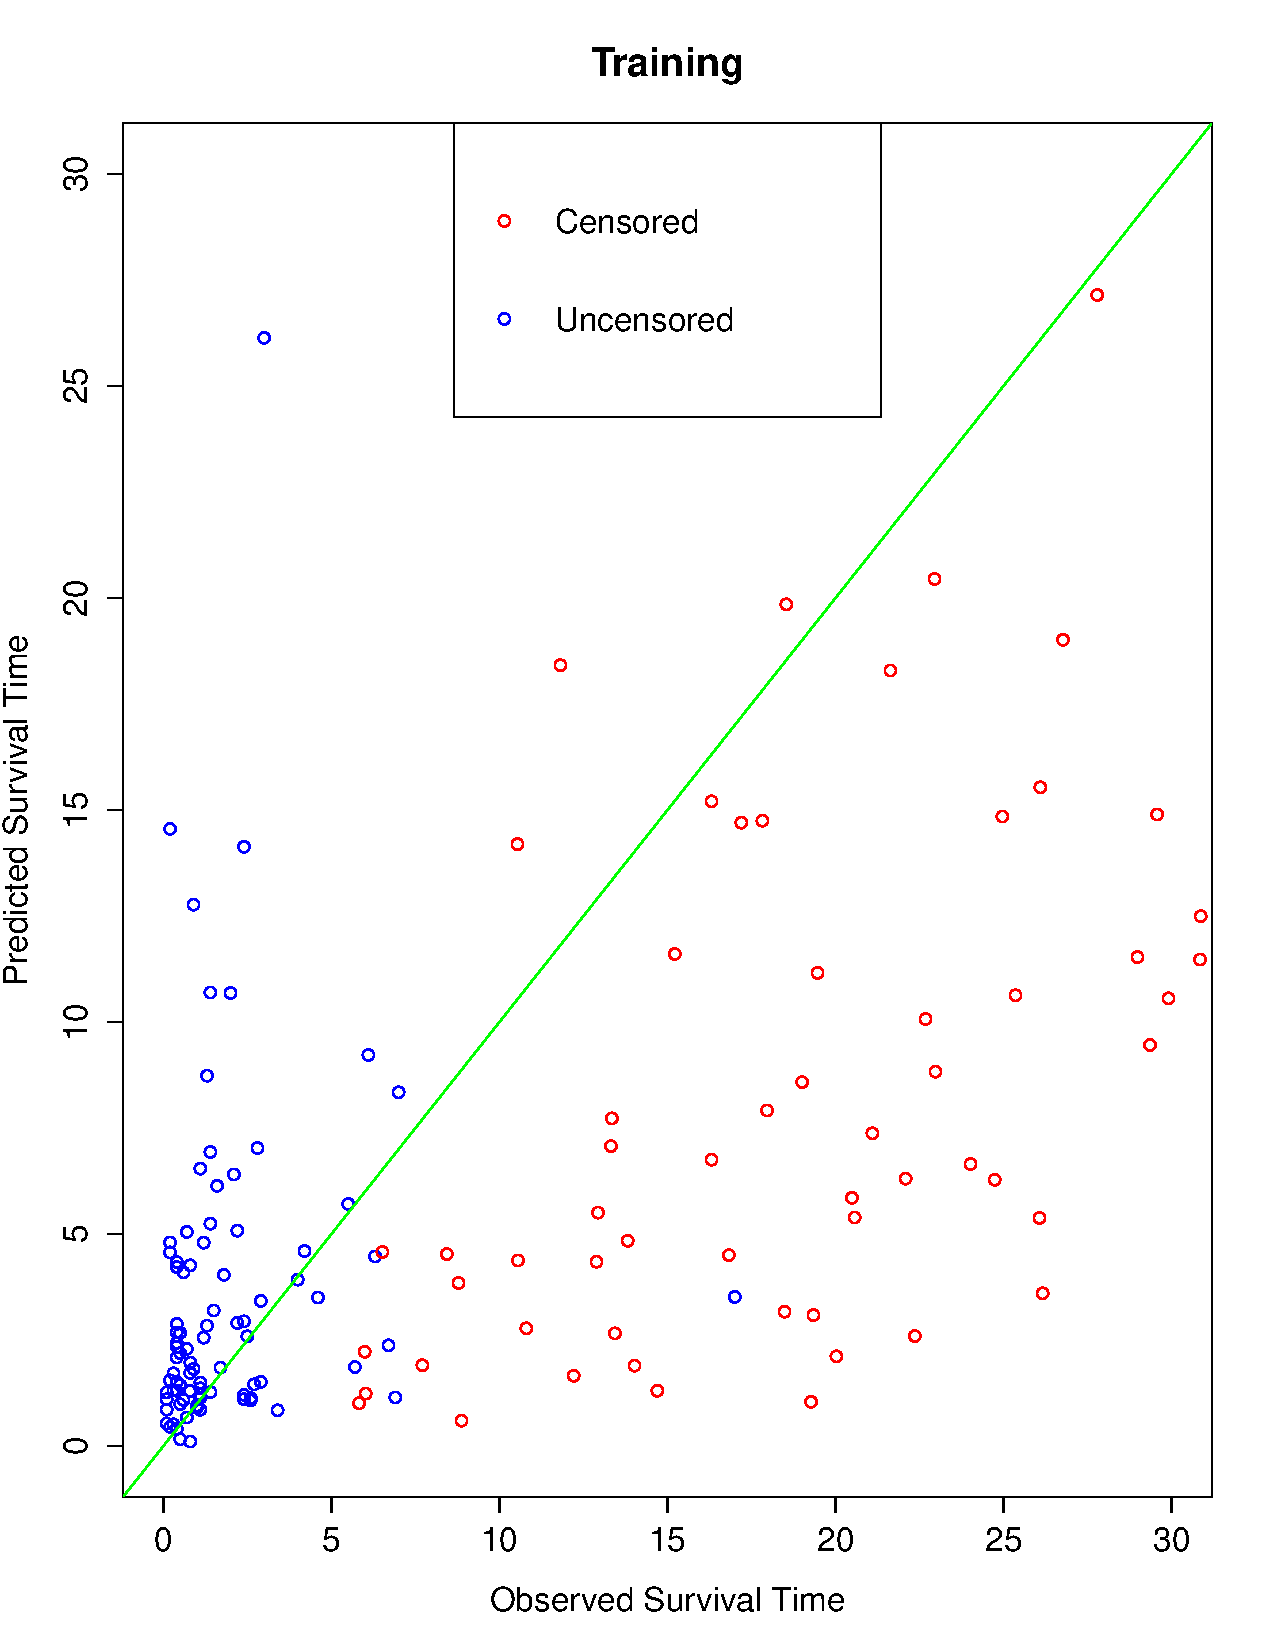
\includegraphics[scale = 0.15]{pred_train.pdf}
	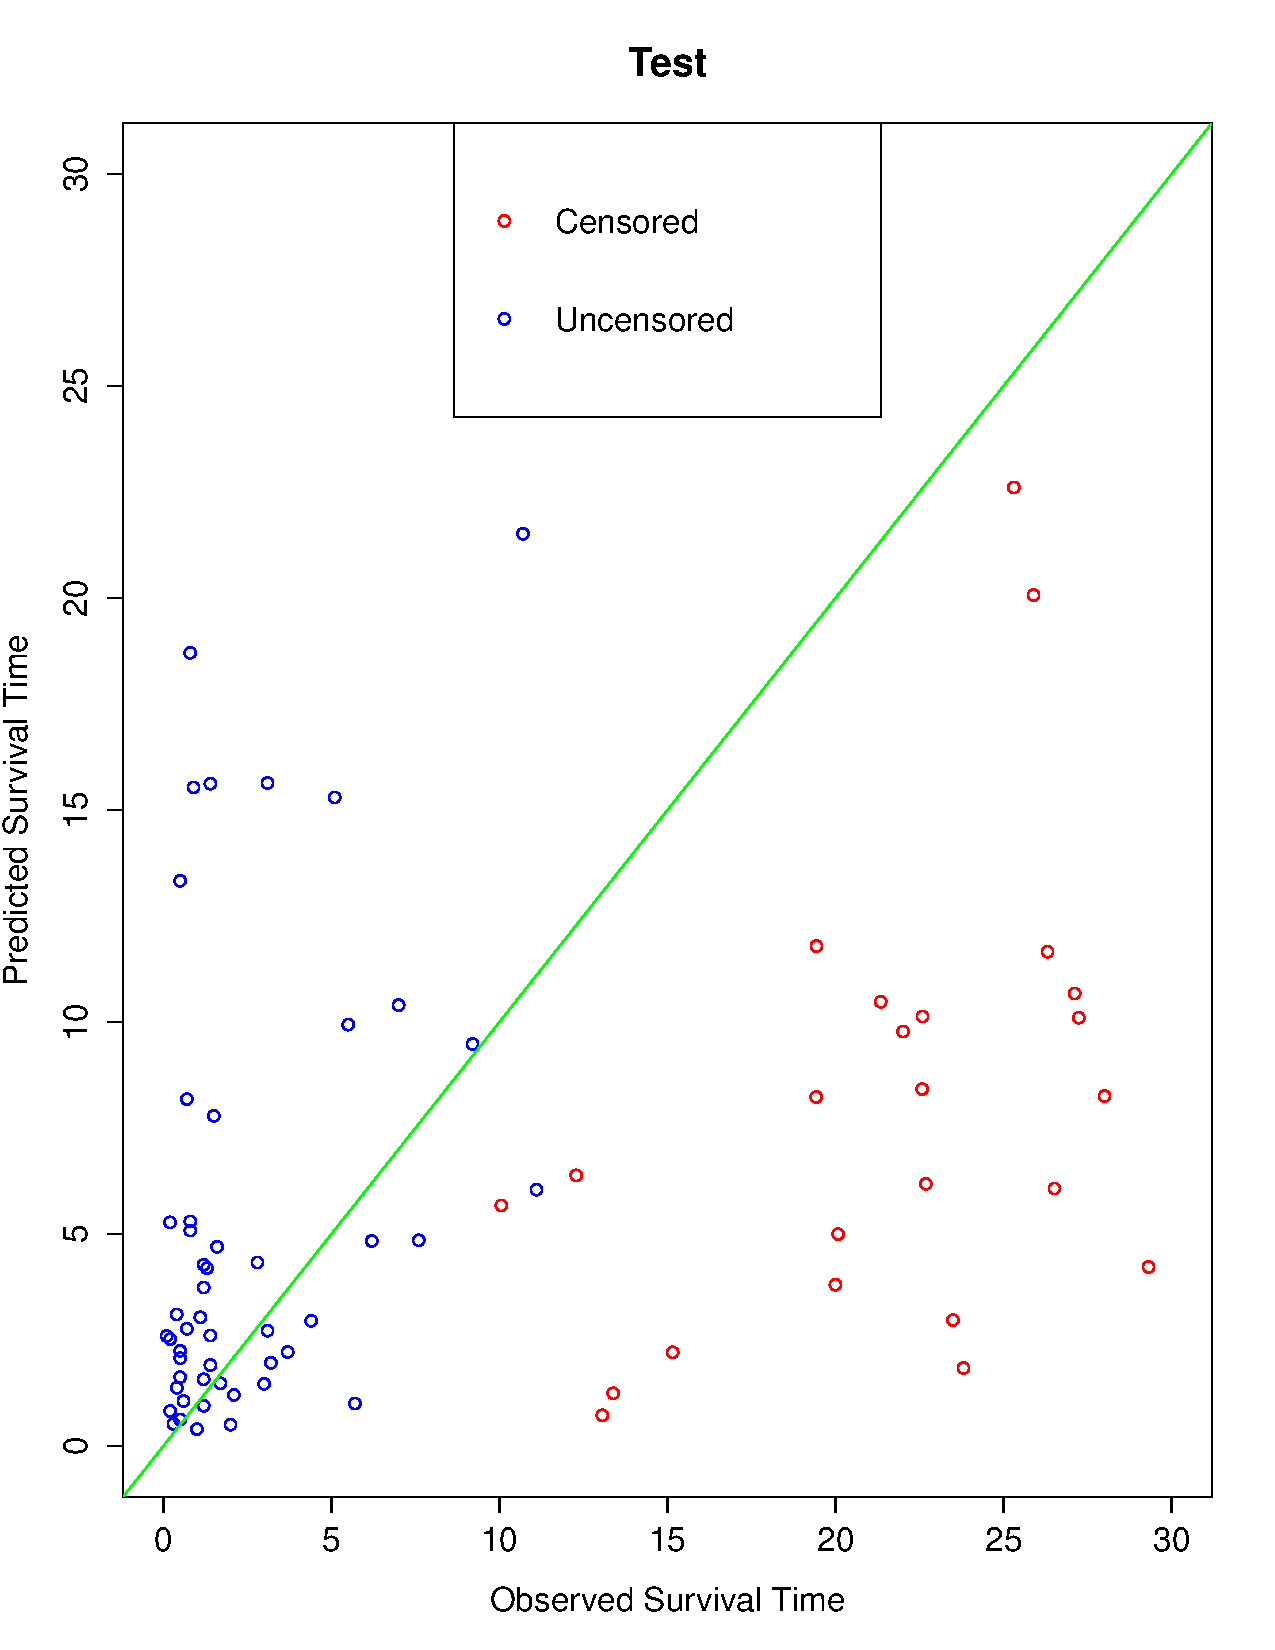
\includegraphics[scale = 0.15]{pred_test.pdf}
    \centering
    
    Figure 1: Observed vs Predicted Survival Times, Unweighted Latent Factor Model
    
    \vspace{2 mm}

\begin{tabular}{|c|c|c|c|}
\hline	
Model & Training & Test \\
\hline\hline
Unweighted & 10.395 & 11.376 \\
\hline
Weighted (w = 1) & 22.314 & 20.874 \\
\hline
Weighted (w = 50) & 49.651 & 19.838 \\
\hline
Weighted (w = 100) & 115.056 & 26.850 \\
\hline
\end{tabular}


Table 1: Comparison of Root Mean Squared Errors

\vspace{2 mm}   

    \end{minipage}
};

\node[fancytitle, right=10pt] at (box.north west) {Result};
\end{tikzpicture}


\begin{tikzpicture}
\node [mybox] (box){%
    \begin{minipage}{0.3\textwidth}
	The unweighted latent factor model is the best performing of all; however, it is likely to underestimate the imputed data (Figure 1). This can be due to the limitation of the model or the inadequacy of single imputation. 

\vspace{2mm} 

	The two features we tried to implement in the weighted models are upweighting the likelihood contribution of survival times, and enforcing sparsity by applying restricting priors to factor loadings. The reason they did not give satisfactory results can be due to imperfect tuning process (tuning parameters include number of latent factors, weighting, and sparsity control) and the size of data set.

\vspace{2mm} 

	Note that for the weighted models, training RMSEs are higher than test RMSEs. One possible reason is that some extreme predictions blow up errors, and the training set has more extreme predictions because they have more data points than the test set.
    \end{minipage}
};

\node[fancytitle, right=10pt] at (box.north west) {Discussion};
\end{tikzpicture}

\end{multicols*}
\end{document}